\chapter{Performance Evaluation and Results}\makeatletter\def\@currentlabel{4}\makeatother
\label{chap4}
\lhead{\textbf{CHAPTER 4.} \textit{Performance Evaluation and Results}}

This chapter explains \textit{how} we measure the performance of \textit{zkpoex} and \textit{what} the measurements reveal. Only the execution that runs \textit{inside} the RISC Zero zkVM is timed; the subsequent on-chain Groth16 verification is ignored because its cost depends on gas price and network congestion. Every run is profiled with the official RISC Zero workflow\cite{risc0_profiling}, and the resulting data are rendered as Brendan Gregg-style flame graphs for fast, visual hotspot discovery\cite{gregg_cpu_flamegraphs}.

\section{Evaluation Metrics}
This section defines the very small set of numbers and pictures we rely on when comparing different proofs. In the next subsections, we will see all the evaluation metrics calculated following the \textit{Guest Profiling Guide} from the Risc Zero Docs \cite{risc0_profiling}. 

\subsection{Quantitative metric}
As a main quantitative metric, there are the \textit{total cycles}: the sum of guest and kernel cycles, which serves as the single numeric predictor of prover cost, because the RISC Zero prover scales linearly with this length \cite{risc0_optimization}.  
Wall-clock seconds are logged for context, but fluctuate with host frequency and
cache hierarchy, so they are never used for cross-machine comparisons.

\subsection{Flame graph metric}
A flame graph is an SVG where each rectangle represents a stack frame sampled at every cycle; the \textit{width} of the box equals the fraction of total cycles spent in that frame, and the x-axis therefore aggregates 100\% of runtime \cite{gregg_cpu_flamegraphs}. The y-axis shows call-stack depth, making deep towers easy to spot as recursive or interpreter loops\cite{gregg_cpu_flamegraphs}. Colours are random warm tones with no semantics. With the flame graph, all the data is on screen at once, and the hottest code-paths are immediately obvious as the widest functions. The built-in \texttt{pprof} viewer adds hover tool-tips, zoom, regex search, and red/blue differential mode for regressions\cite{pprof_flamegraph,gregg_diff_flamegraphs}.

\section{Profiling Methodology}
This section records the exact steps needed to reproduce the profiles shown later. We calculated a \textit{profile} for each case study in the \ref{case_studies} Section in Chapter 3. Proof generation times will be shown in the next section \ref{proof_analysis}.

\subsection{Prerequisites}  
As indicated in \cite{risc0_profiling}, the main prerequisite for viewing flame graphs and all related metrics is Go. So you need to install it because it bundles with it the \textit{pprof} tool. Obviously, all the prerequisites of the Risc Zero zkVM are necessary.

After installing Go, you need to set all these variables as below:

\begin{verbatim}
RISC0_PPROF_OUT=./profile.pb \
RISC0_DEV_MODE=1 \
RUST_LOG=info 
\end{verbatim}

The variable \texttt{RISC0\_DEV\_MODE=1} skips real proving so the profile is
generated in seconds\cite{risczero_dev_mode}. When this flag is enabled the zkVM runs the guest exactly as in production but returns a \emph{fake receipt} instead of executing the heavyweight STARK and Groth16 pipelines.

Generating the cryptographic proof is unnecessary at this stage because we are interested solely in the guest execution time and the cycle distribution recorded inside the zkVM trace; both are fully captured before the heavy STARK computation and Groth16 compression begin. Dev-mode, therefore, produces an identical flame graph and cycle count in a fraction of the time, giving an accurate snapshot of run-time performance without incurring the extra cost of creating a final, on-chain-ready proof.

After setting the variables, simply run the \texttt{just} command to generate an exploit proof for any example you want to demonstrate (see Listing \ref{example_just} as an example, in this case for the \textit{BasicVulnerable} case study), and the \texttt{profile.pb} file will be generated and saved in the location indicated in the \texttt{RISC0\_PPROF\_OUT} variable.

\begin{figure}[h]
  \centering
  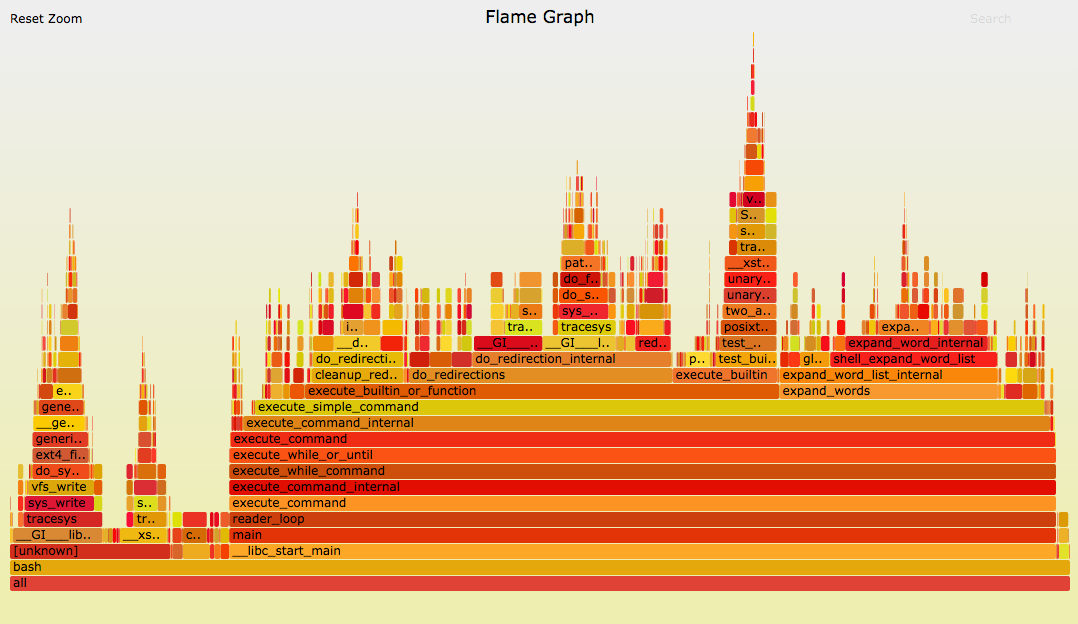
\includegraphics[width=\linewidth]{Images/Chap4/cpu-bash-flamegraph.png}
  \caption{Interactive flame graph generated by \texttt{pprof}.}
  \label{fig:flamegraph_example}
\end{figure}
\subsection{Visualisation}  
Once the profiling run has produced its \texttt{profile.pb}, the file can be inspected directly with the web-UI bundled into \texttt{pprof}.  

Launching
\begin{verbatim}
go tool pprof -http=127.0.0.1:8000 ./profile.pb
\end{verbatim}
starts a local server on port 8000; visiting the indicated URL opens an interactive SVG that embeds every cycle of execution. The interface is intentionally minimal yet powerful: moving the cursor across the graph reveals, in a tooltip, the fully qualified function name together with the exact number of cycles it consumed, so the dominant hot spots become obvious without leaving the page. Clicking any rectangle zooms the view so that the selected frame now fills the width of the browser window, effectively filtering the graph to the subtree beneath that call; a breadcrumb trail at the top of the page lets you ascend the stack again with a single click.  

If you have two profiles, for example, before and after an optimisation, you can
feed both \emph{protobufs} to the same \texttt{pprof} command; the viewer then
switches automatically to differential mode and colours frames according to
how much their share of total cycles has grown or shrunk, a visual aid that
makes regressions stand out immediately.  

Because the flame graph is a self-contained SVG, it can be downloaded with the
browser’s “Save” dialog; no external CSS or JavaScript is required, so anyone
can view the graph without installing additional tools \cite{pprof_flamegraph,gregg_diff_flamegraphs}.

In Figure \ref{fig:flamegraph_example}, an example of a flame graph.

\section{Profiling Analysis} \label{proof_analysis}
This section applies the profiling workflow to the three exploits introduced in ~\ref{case_studies} Section in Chapter 3, concentrating on the \texttt{run\_evm} frame because all vulnerability logic executes inside the EVM interpreter embedded in the zkVM. For each case study, we report the total guest cycle budget, discuss how many of those cycles fall under \texttt{run\_evm}, and highlight the most expensive descendants. 

The table below converts the raw “guest-cycle” counters emitted by
\texttt{pprof} into an \emph{ideal} execution time via
\[
\text{time}_{\mathrm{guest}}
       =\frac{\text{cycle count}}{f_{\mathrm{CPU}}},
       \qquad f_{\mathrm{CPU}}=2.0\times10^{9}\;\text{Hz}
\]
($f_{\mathrm{CPU}}$ is the base clock of a Ryzen 7 4700U). Because one guest tick is mapped to a single \texttt{rv32im} instruction, the division gives a \textit{lower-bound} latency: stalls, cache misses, and the subsequent STARK /
Groth16 stages are \emph{not} included here.  For instance, the \textit{Basic Vulnerable} run consumes \(702\,098\) ticks, which yields \(\tfrac{702\,098}{2\cdot10^{9}}\approx0.35\;\text{ms}\).

\begin{table}[h]
\centering
\begin{tabular}{|l|c|c|c|}
\hline
\textbf{Case study} & \textbf{total cycles} & \textbf{\texttt{run\_evm} share} & \textbf{guest time (ms)\textsuperscript{*}} \\\hline
Basic Vulnerable      & \(9.99\times10^{5}\) & 70.3\,\% & 0.35 \\\hline
Unchecked Arithmetic  & \(4.05\times10^{5}\) & 75.9\,\% & 0.15 \\\hline
Reentrancy Drain      & \(1.81\times10^{6}\) & 91.2\,\% & 0.82 \\\hline
\end{tabular}
\caption{Cycle budget, dominance of \texttt{run\_evm}, and ideal guest
latency on an AMD Ryzen 7 4700U.}
\label{tbl:proofstats}
\begin{minipage}{0.9\linewidth}
\smallskip
\textsuperscript{*}\,\emph{Guest time} covers only the RISC-V trace that executes the EVM logic; it excludes circuit interpolation, FRI commitment, Groth16 compression, and I/O. 
\end{minipage}
\end{table}



\subsection{BasicVulnerable Case Study Evaluation}
Figure~\ref{fig:flame_basic} shows that \texttt{run\_evm} consumes approximately 70\,\% of all cycles. Inside that frame, most time is spent hashing the pre-state (\texttt{context\_state}) and calculating program-spec digests, followed by the Keccak \texttt{p1600} primitive. The actual EVM execution path (\texttt{transact\_call} \(\rightarrow\)\texttt{Runtime::run}) is comparatively shallow because the exploit issues a single value-bearing \texttt{CALL} that forwards the contract’s entire balance to \texttt{address(0)}; once the transfer is executed, no further storage writes or complex gas-cost paths are triggered, so the interpreter exits quickly.

\begin{figure}[h]
  \centering
  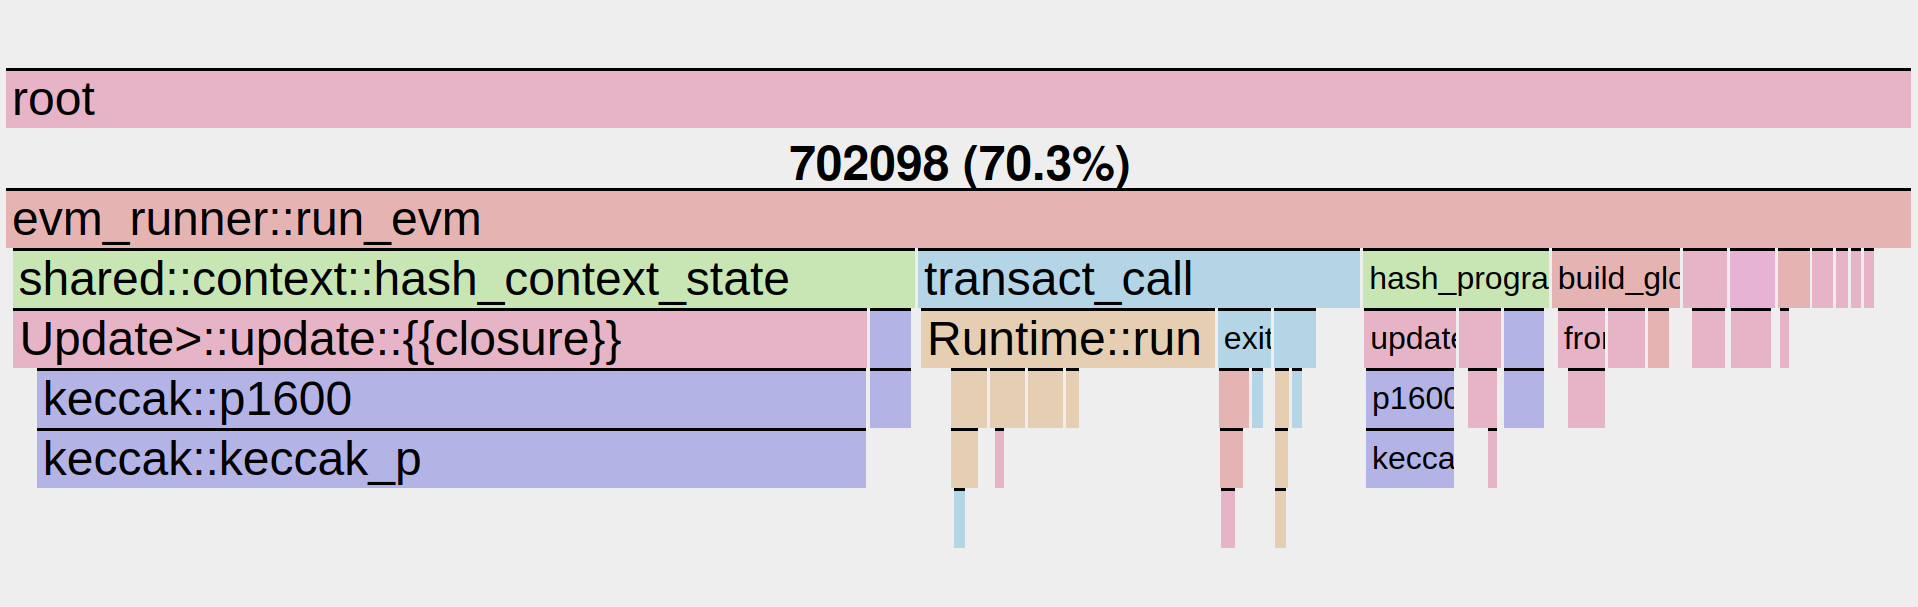
\includegraphics[width=\linewidth]{Images/Chap4/basicVulnerable_fg.png}
  \caption{Flame graph for the \textit{BasicVulnerable} logical exploit.}
  \label{fig:flame_basic}
\end{figure}

\subsection{Unchecked Arithmetic Case Study Evaluation}
Figure~\ref{fig:flame_overflow} confirms that \texttt{run\_evm} still dominates the trace, yet its internal profile differs markedly from the Basic case. The interpreter loop is wider even though the total cycle budget is smaller, because the exploit executes two storage touching opcodes: one \texttt{SLOAD} to fetch \texttt{balance} and one \texttt{SSTORE} to write back the wrapped value. Each storage access triggers the Merkle-Patricia-Trie machinery inside \texttt{StackExecutor::transact\_call}, which explains the pronounced block of hashing just beneath the loop.  The unchecked subtraction itself appears as a narrow frame; the real cost lies in updating the trie and recalculating the slot digest.  A \texttt{run\_evm} share of 75.9\%, therefore, means JSON decoding and context hashing are amortised over fewer total cycles, making the interpreter’s storage paths the clear target for future optimisation.


\begin{figure}[h]
  \centering
  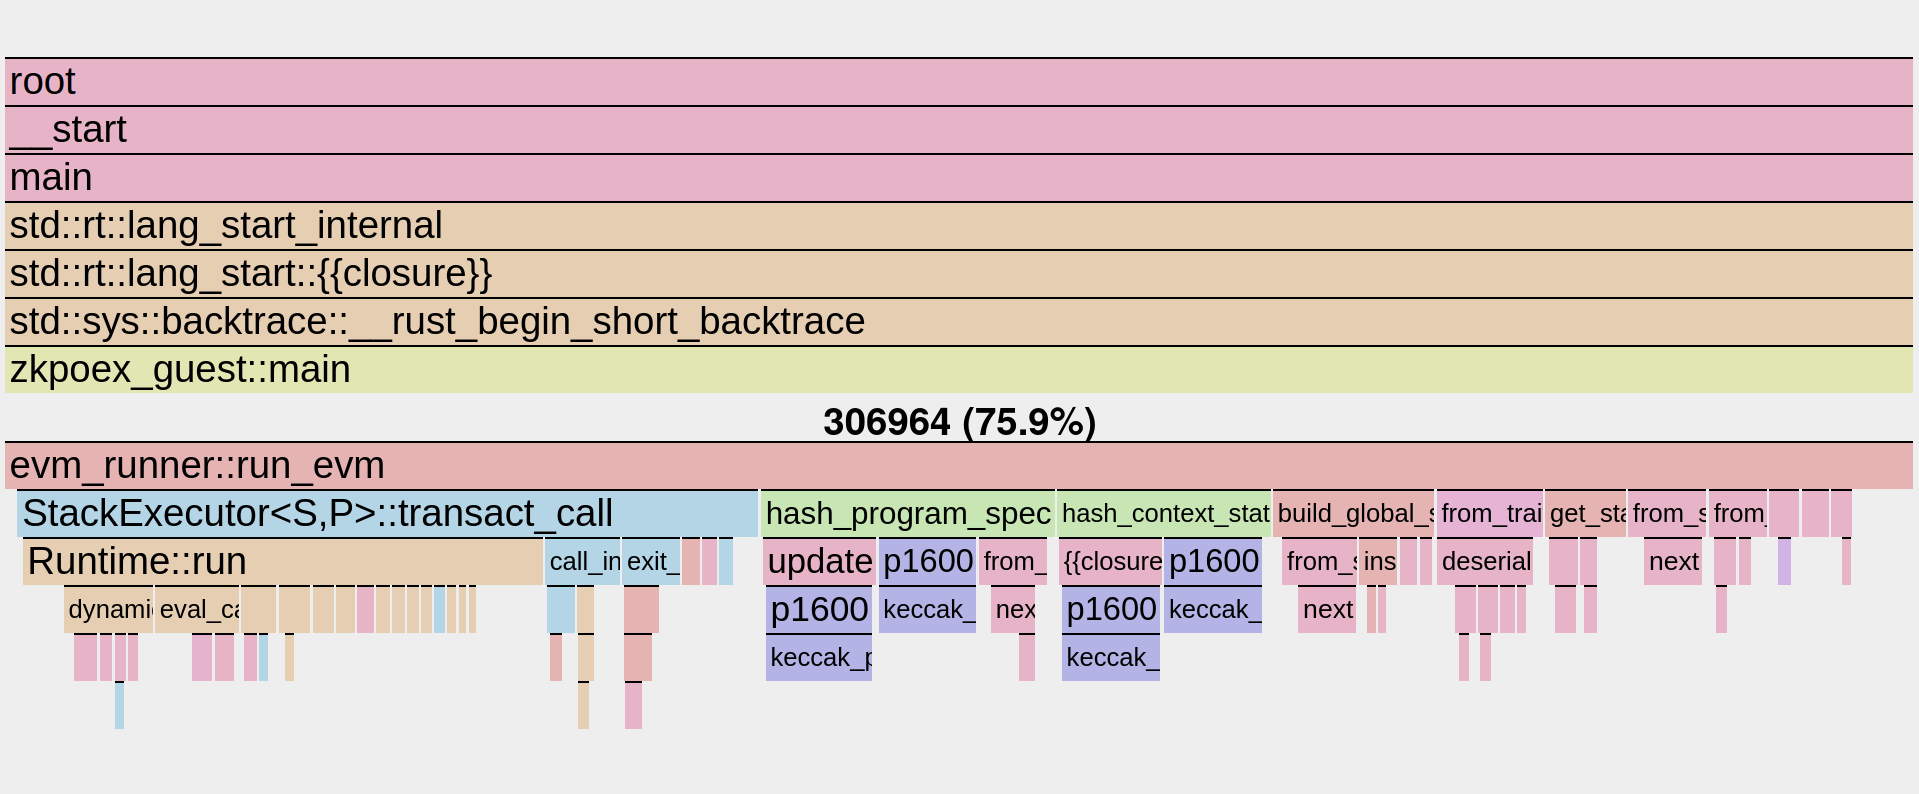
\includegraphics[width=\linewidth]{Images/Chap4/overUnderFlowVulnerable_fg.png}
  \caption{Flame graph for the \textit{Unchecked Arithmetic} overflow exploit.}
  \label{fig:flame_overflow}
\end{figure}

\subsection{Reentrancy Drain Evaluation}
Figure~\ref{fig:flame_reentrancy} shows that \texttt{run\_evm} dominates 91.2\,\% of the total trace, far higher than in the other two runs. The reason is visible in the shape of the graph: every external \texttt{CALL} to the attacker’s fallback re-enters \texttt{withdrawETH}, so the interpreter never unwinds to the host; instead, it spawns a nested EVM invocation that appears as another wide block under the parent \texttt{eval} frame.  Because the balance mapping is cleared only after the transfer, each callback observes a positive balance and triggers yet another \texttt{CALL}, producing a forest of stacked frames.  The dynamic gas-cost routine (\texttt{dynamic\_opcode\_cost}) forms a distinct tower to the right, reflecting the variable cost charged for cold versus warm storage slots on every entry.  Even with this heavier control flow, the timing scales linearly: the trace contains roughly twice the cycles of \textit{Basic Burn} and takes roughly twice as long to execute, confirming that the total cycle metric reliably forecasts wall clock performance in reentrancy scenarios.

\begin{figure}[h]
  \centering
  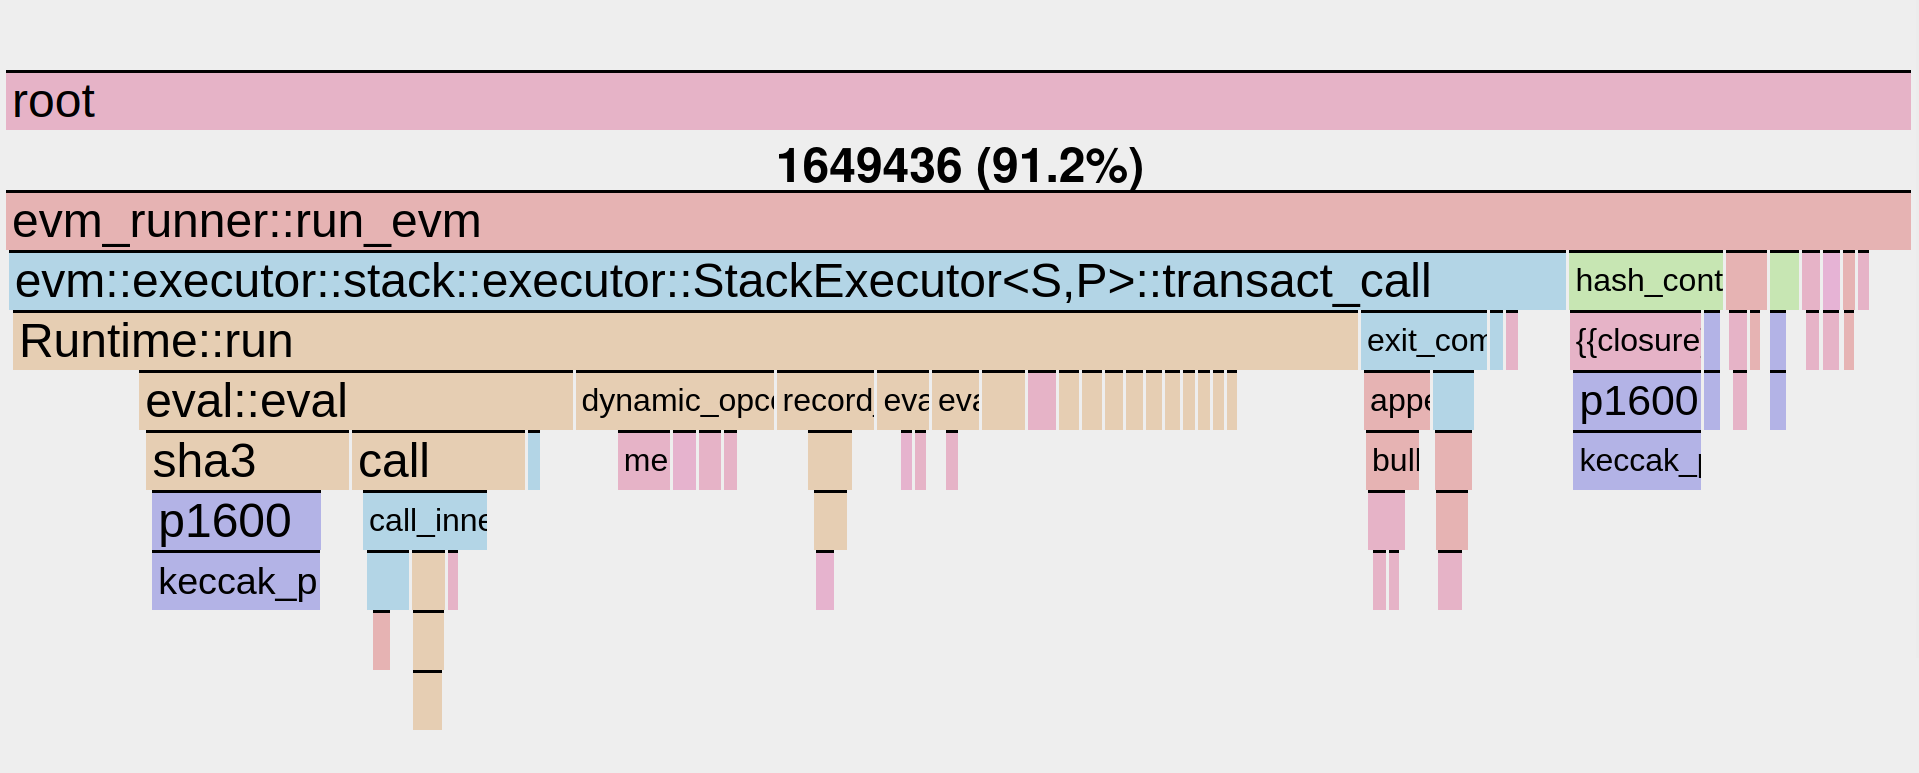
\includegraphics[width=\linewidth]{Images/Chap4/reentrancyVulnerable_fg.png}
  \caption{Flame graph for the \textit{Reentrancy Drain} exploit.}
  \label{fig:flame_reentrancy}
\end{figure}
%The large beige region under \texttt{StackExecutor::transact\_call} represents repeated \texttt{CALL} handling.
